\documentclass{article}
\usepackage{graphicx} % Required for inserting images
\usepackage{authblk} % Required for author affiliations
\usepackage{indentfirst} % Indent first paragraph of sections
\usepackage{amssymb} % For mathematical symbols
\usepackage{amsthm} % For theorem environments
\usepackage{amsmath} % For advanced math typesetting
\usepackage[hidelinks]{hyperref}
\usepackage{enumitem}
\usepackage{pgfplots} % For plots
\pgfplotsset{compat=1.18} % Set compatibility level
\usepackage{tikz} % For drawing shapes
\newtheorem{theorem}{Theorem}
\newtheorem{corollary}{Corollary}[theorem]
\newtheorem{lemma}[theorem]{Lemma}
\newtheorem{definition}{Definition}
\newtheorem{problem}{Problem}
\newtheorem{solution}{Solution}
\newtheorem*{example}{Example}
\newtheorem{remark}{Remark}
\reversemarginpar
\begin{document}
%------- Title page   -----------
\title{MATH 223: Linear Algebra}
\author{William Homier}
\affil[1]{McGill University Physics, 3600 Rue University, Montréal, QC H3A 2T8, Canada}
\date{January \(5^{th}\), 2026}
\setcounter{Maxaffil}{0}
\renewcommand\Affilfont{\itshape\small}
\maketitle

%------- Abstract -----------
\noindent\rule{\textwidth}{0.4pt}
\thispagestyle{empty}
\begin{abstract}

\end{abstract}
\noindent\rule{\textwidth}{0.4pt}
\clearpage

%------- Table of Contents -----------
\thispagestyle{empty}
\hypersetup{
    citecolor=black,
    filecolor=black,
    linkcolor=black,
    urlcolor=black
}
\tableofcontents
\clearpage

%------- introduction -----------
\setcounter{page}{1}
\section{Introduction}

\section{Prerequisite knowledge}
\subsection{Notation}
\subsubsection{Sets}
Sets are a grouping of objects.
\begin{itemize}
    \item \(\mathbb{N}\) is the set of natural numbers: (0, 1, 2, 3, ...).
    \item \(\mathbb{Z}\) is the set of integers: (..., -3, -2, -1, 0, 1, 2, 3, ...).
    \item \(\mathbb{Q}\) is the set of rational numbers (numbers that can be expressed as a fraction of two integers): \(\mathbb{Q} = {\frac{a}{b} | a,b \in \mathbb{Z}, b \neq 0}\).
    \item \(\mathbb{R} =\) all rational + all irrational numbers.
    \item \(\mathbb{C} = \{x + iy | x,y \in \mathbb{R}\}\), basically: \(\mathbb{C} =\) all real (\(\mathbb{R}\)) + all imaginary numbers (\(i\)), where \(i\) is defined to be a root of \(x^2 + 1\), which is \(i \subseteq \sqrt{-1}\).
\end{itemize}
We have the following relationships between sets:
\[\mathbb{N} \subseteq \mathbb{Z} \subseteq \mathbb{Q} \subseteq \mathbb{R} \subseteq \mathbb{C}\]
\subsubsection{Symbols}
We will be using the following symbols:
\begin{itemize}
    \item \(\subseteq\) means "is a subset of or equal to".
    \item \(\subset\) means "is a subset of" or "is contained in", it could also mean the same thing as \(\subseteq\), but not all the time.
    \item \(\forall\) means "for all".
    \item \(\exists\) means "there exists".
\end{itemize}

\subsection{Complex Algebra}
\subsubsection{Complex Numbers}
A complex number is of the form: \(z = x + iy\) where \(x,y \in \mathbb{R}\) and \(i\) is the imaginary unit such that \(i^2 + 1 = 0\).
\begin{theorem}[Fundamental Theorem of Algebra]
    Any polynomial\footnote{Polynomial is a function such as: \(f = a_n x^n + a_{n-1}x^{n-1} + ... + a_1 x + a_0\) where \(a_i \in \mathbb{R}\) or \(\mathbb{C}\) and \(n \in \mathbb{N}\).} \(f\) (except constant functions) has a root in \(\mathbb{C}\).
\end{theorem}
\begin{remark}
    If we have a polynomial \(f\) of degree \(n\), then it has \(n\) roots, where each root can have a multiplicity\footnote{The multiplicity of a root represents how many times the root occurs in the polynomial.}. For example, if we have a polynomial \((x-1)^2\), it has a degree of 2 but only one root, which is 1, with a multiplicity of 2. This means that the root 1 appears twice in the polynomial.
\end{remark}
We can factorize a polynomial in the form of \(f = a_n x^n + ... + a_1 x + a_0\) into a linear factor: \(f = a(x - z_1)(x - z_2)...(x - z_n)\) where \(z_i\) are the roots of \(f\) in \(\mathbb{C}\).\\\\
Using the FTA for a function such as \(f = a_nx^n + ... + a_1 x + a_0\), we can say that the FTA implies that \(f\) has a root \(f(z) = 0\).
\subsubsection{Complex Operations}
\label{subsec:CO}
We can define operations on complex numbers as follows:
\begin{itemize}
    \item Addition: \(z + z' = (x + x') + i(y + y')\), where \(x,x',y,y' \in \mathbb{R}\).
    \item Multiplication: \(zz' = (x + iy)(x' + iy') = (xx' - yy') + i(xy' + yx')\).
    \item Inverse: \(\frac{1}{z} = \frac{\overline{z}}{z\overline{z}} = \frac{x - iy}{x^2 + y^2} = \frac{x}{x^2 + y^2} + i\frac{-y}{x^2 + y^2}\)
\end{itemize}
From the definition of inverse, we can see that for any complex number \(z\), its inverse \(\frac{1}{z}\) is also a complex number. For example, take \(z = 1 + i\), where \(x = y = 1\), from the definition of inverse, we can conclude that: \[\frac{1}{1 + i} \in \mathbb{C}\]
\subsubsection{Complex Conjugate}
A complex conjugate is a way to "flip" the imaginary part of a complex number. For example, if we have a complex number \(z = x + iy\), then the complex conjugate of \(z\) is \(\overline{z} = x - iy\). Some basic properties of complex conjugates are:
\begin{itemize}
    \item \(\overline{z} = z\)
    \item \(\overline{z + z'} = \overline{z} + \overline{z'}\)
    \item \(\overline{z \cdot z'} = \overline{z} \cdot \overline{z'}\)
\end{itemize}

\subsubsection{Geometric and Polar Form of Complex Numbers}
\marginpar{January 09, 2026.}

\begin{definition}[Geometric interpretation]
    Every complex number \(z = x + iy\) can be identified with a point \((x,y)\) in the plane, called the \emph{complex plane}. This allows us to study complex numbers using geometry.
\end{definition}

\begin{center}
\begin{tikzpicture}[scale=2]
% Axes
\draw[->] (-1.4,0)--(1.4,0) node[right]{$x$};
\draw[->] (0,-1.4)--(0,1.4) node[above]{$y$};

% Unit circle
\draw (0,0) circle(1);

% Point z = x+iy
\coordinate (Z) at (0.8,0.6);
\draw[fill] (Z) circle(0.02) node[above right] {$z=x+iy$};

% Projections
\draw[dashed] (Z) -- (0.8,0) node[below] {$x$};
\draw[dashed] (Z) -- (0,0.6) node[left] {$y$};

% Horizontal from y-axis and vertical from x-axis
\draw (0,0.6) -- (Z);
\draw (0.8,0) -- (Z);

% Radius
\draw (0,0) -- (Z);

\end{tikzpicture}
\end{center}

\[\mathbb{C} = \{x + iy \mid x,y \in \mathbb{R}\}.\]

\begin{definition}[Modulus]
    The modulus of a complex number \(z\) is defined by
    \[|z| = \sqrt{z\overline{z}} = \sqrt{x^2 + y^2}.\]
    Geometrically, \(|z|\) is the distance from the origin to the point \((x,y)\).
\end{definition}
We can rewrite the definition of the unit circle as follows:
\[S' = \{(x,y) \in \mathbb{R}^2 : x^2 + y^2 = 1\} = \{ z \in \mathbb{C} : |z| = 1\}.\]
Thus, \(S'\) is the \emph{unit circle} in the complex plane.

\begin{definition}[Powers of \(i\)]
\begin{center}
\begin{tabular}{c|cccccc}
k & 0 & 1 & 2 & 3 & 4 & 5 \\
\hline
$i^k$ & 1 & i & -1 & -i & 1 & i
\end{tabular}
\end{center}
\end{definition}

\begin{definition}[Geometric meaning of multiplication]
    Multiplying by a complex number \(z\) corresponds geometrically to
    \[\begin{cases}\text{a rotation by some angle } \theta,\\\text{a rescaling by the factor } |z|.\end{cases}\]
\end{definition}

\begin{definition}[Polar coordinates]
    Instead of describing a point by \((x,y)\), we may describe it using polar coordinates \((r,\theta)\), where \(r = |z|\) is the distance to the origin and \(\theta\) is the angle with the positive \(x\)-axis.
\end{definition}
\begin{example}
    \begin{center}
    \begin{tikzpicture}[scale=2]
    % Axes
    \draw[->] (-1.4,0)--(1.4,0) node[right]{$x$};
    \draw[->] (0,-1.4)--(0,1.4) node[above]{$y$};

    % Point
    \coordinate (Z) at (0.9,0.5);
    \draw[fill] (Z) circle(0.02) node[above right] {$(x,y)$};

    % Lines
    \draw (0,0) -- (Z) node[midway, above] {$r$};
    \draw[dashed] (Z) -- (0.9,0);
    \draw[dashed] (Z) -- (0,0.5);

    % Angle theta
    \draw (0.4,0) arc (0:29:0.4);
    \node at (0.45,0.12) {$\theta$};

    \end{tikzpicture}
    \end{center}

    \[x = r \cos(\theta), \quad y = r \sin(\theta).\]
\end{example}


\begin{definition}[Polar and exponential form]
    \[z = x + iy = r \cos(\theta) + ir \sin(\theta) = r(\cos(\theta) + i \sin(\theta)) = re^{i\theta}.\]
\end{definition}

\begin{definition}[Euler's formula]
    Euler's formula gives
    \[e^{i\theta} = \cos(\theta) + i \sin(\theta).\]
\end{definition}

\begin{definition}[Multiplication in polar form]
    \[z = re^{i\theta}, \quad z' = r'e^{i\theta'}, \quad zz' = rr'e^{i(\theta + \theta')}.\]
\end{definition}
\begin{example}
    \[(1 + i)^{32} = (\sqrt{2}e^{i\pi/4})^{32} = (\sqrt{2})^{32} e^{i8\pi} = 2^{16}(\cos 8\pi + i \sin 8\pi) = 2^{16}.\]
\end{example}


\begin{definition}[\(n^{\text{th}}\) roots]
    An \(n^{\text{th}}\) root of \(z\) is a complex number \(w\) such that
    \[w^n = z.\]
\end{definition}

\begin{definition}[Roots of unity]
    The \(n^{\text{th}}\) roots of unity are the solutions of
    \[w^n = 1, \quad w \in \mathbb{C}.\]
    Geometrically, they lie on the unit circle \(|w|=1\).
    \begin{center}
    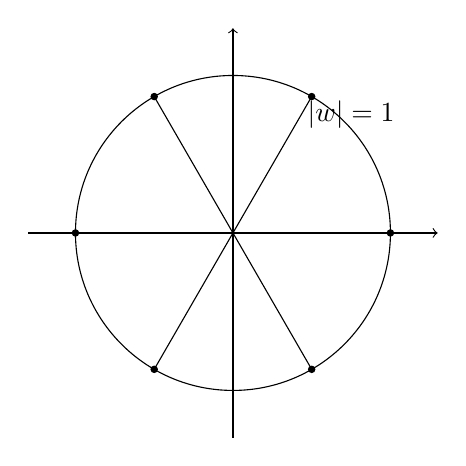
\begin{tikzpicture}[scale=2]
    % Axes
    \draw[->] (-1.3,0)--(1.3,0);
    \draw[->] (0,-1.3)--(0,1.3);

    % Unit circle
    \draw (0,0) circle(1);

    % Example: n = 6 roots
    \foreach \k in {0,1,2,3,4,5}{
    \coordinate (P\k) at ({cos(60*\k)},{sin(60*\k)});
    \draw[fill] (P\k) circle(0.02);
    \draw (0,0) -- (P\k);
    }

    \node at (0.75,0.75) {$|w| = 1$};
    \end{tikzpicture}
    \end{center}

    \[1 = e^{i2\pi k}, \quad k \in \mathbb{Z},\]
    \[w_k = e^{i2\pi k/n}, \quad w^n = (e^{i2\pi/n})^n = e^{i2\pi} = 1.\]
\end{definition}


\section{Basic Algebraic structures}
"Let V be a vector space over a field K"

\subsection{Invertibility}
\begin{definition}[Condition for Invertibility]
    Let \(A \in M\) be an \(n \times n\) matrix, and suppose that there exists an \(n \times n\) matrix \(B\) such that \(AB = I_n\) or \(BA = I_n\). Where \(I_n\) is the \(n \times n\) identity matrix\footnote{An identity matrix is a square matrix with 1s on its main diagonal and 0s everywhere else. It represents no change in linear transformations, and it's used in finding matrix inverses.}$\begin{bmatrix}1&0&0&0\\0&1&0&0\\0&0&...&0\\0&0&0&1\end{bmatrix}$. Then A is invertible, and \(B = A^{-1}\).
\end{definition}

\begin{remark}
    If \(A\) is invertible, then \(A^{-1}\) exists and is unique\footnote{Unique means there is exactly one such element.}.
\end{remark}

To determine if an element \(A\) in a set with multiplication \(M\) is invertible, we can use the following examples:
\begin{example}
    Let \(M = \mathbb{Z} = \{...-2,-1,0,1,2,...\}\) and \(A = 2\). Is \(A\) invertible in \(M\)?\\
    Solution: No, because \(\frac{1}{2} \notin \mathbb{Z}\).
\end{example}
\begin{example}
    Let \(M = \mathbb{R}\) and \(A = 2\), is \(A\) invertible in \(M\)?\\
    Solution: Yes, because \(\frac{1}{2} \in \mathbb{R}\).
\end{example}
\begin{example}
    Is \(1 + i\) invertible in \(\mathbb{C}\)?\\
    Solution: Yes, using our previous definition of inverse (\ref{subsec:CO}), we get that \[\frac{1}{1 + i} = \frac{1 - i}{2} \in \mathbb{C}.\]
\end{example}

\subsection{Ring}
\begin{definition}
A ring is a set \(R\) with the following properties:
\begin{enumerate}
    \item \(R\) is an abelian group under addition.
    \item \(R\) is a monoid under multiplication.
    \item The distribution law holds: \(a(b + c) = ab + ac\) for all \(a,b,c \in R\).
\end{enumerate}
\end{definition}
More informally, a ring is a set with two operations (addition and multiplication) that satisfy certain properties.\\
The main example of a ring is the set of integers \(\mathbb{Z}\).
\subsection{Field}
\begin{definition}
A field is a commutative ring in which every element is invertible.
\end{definition}
The main example of a field is the real numbers \(\mathbb{R}\) or the complex numbers \(\mathbb{C}\). Mathematically, \(K = \mathbb{R}\) or \(\mathbb{C}\), where \(K\) is the field.\\
In the following explanation, we will denote \(M\) to be a set with multiplication\footnote{A set of objects where you can multiply any two of them.}.
An example of a set with multiplication is the set of all \(2 \times 2\) complex matrices: \(M = M_2(\mathbb{C})\). Another example is the nonzero set of all real numbers \(\mathbb{R}\) with ordinary multiplication: \(\mathbb{R}^* = \mathbb{R} \setminus \{0\}\).

\begin{problem}
    Construct a field with 2 elements.
\end{problem}
\begin{problem}
    Show that if an inverse of A in \(\mathbb{M}\) exists, then it is unique.
\end{problem}
\begin{problem}
    Let \(K\) be a field. Prove that this matrix $\begin{bmatrix}0&1\\0&0\end{bmatrix}$ \(\in M_2(K)\) is not invertible.
\end{problem}

\section{Vector Spaces}
\marginpar{January 09, 2026.}
\subsection{Cartesian space}
\[\mathbb{R}^n = \begin{cases}
    \begin{pmatrix}
        x_1\\
        \ldots\\
        x_n
    \end{pmatrix} : x_1, \ldots, x_n \in \mathbb{R}
\end{cases}
\]
You can add two vectors:
\[\begin{pmatrix} x_1 \\ \vdots \\ x_n \end{pmatrix} + \begin{pmatrix} y_1 \\ \vdots \\ y_n \end{pmatrix} = \begin{pmatrix} x_1 + y_1 \\ \vdots \\ x_n + y_n \end{pmatrix}\]
Scalar multiplication:
\[\lambda \begin{pmatrix} x_1 \\ \vdots \\ x_n \end{pmatrix} = \begin{pmatrix} \lambda x_1 \\ \vdots \\ \lambda x_n \end{pmatrix}\]
where \(\lambda \in \mathbb{R}\).

A linear combination is a vector \(v\) of the form \(v = \lambda_1v_1 + \ldots + \lambda_nv_n\).

\[\xi((v_1 + 2v_2) + v_3) + v_4\]
Set A inside \(\mathbb{R}^2\)
\(Span(A) =\) all linear combinations of elements in A.

\[
\begin{pmatrix}
    1\\1
\end{pmatrix}
\in \mathbb{R}^2\]
\[A = \begin{cases}
    \begin{pmatrix}
        1\\1
    \end{pmatrix}
\end{cases}\]
Draw a graph with one long diagonal line in the +x, +y and three arrows on the same line showing the vector grows.

\[Span\{r\} = \] line spanned by \(v\)

\section{Appendix}

\section{Solutions}
\begin{solution}
    A field with 2 elements can be constructed as follows:
    Let \(F = \{0, 1\}\) be a set with two elements. We define addition and multiplication operations on \(F\) as follows:
    \begin{itemize}
        \item \(0 + 0 = 0\)
        \item \(0 + 1 = 1\)
        \item \(1 + 0 = 1\)
        \item \(1 + 1 = 0\)
        \item \(0 \times 0 = 0\)
        \item \(0 \times 1 = 0\)
        \item \(1 \times 0 = 0\)
        \item \(1 \times 1 = 1\)
    \end{itemize}
\end{solution}
\begin{solution}
    Suppose \(B\) and \(B'\) are both inverses of \(A\). Then
    \[B = B I = B(AB') = (BA)B' = I B' = B'.\]
    Therefore, \(B = B'\), so the inverse is unique.
\end{solution}
\begin{solution}
    We can answer this problem with proof by contradiction. Let's
    suppose this matrix is invertible. By definition there exists B = $\begin{pmatrix}a&b\\c&d\end{pmatrix}$ such that $\begin{bmatrix}0&1\\0&0\end{bmatrix}$ $\begin{bmatrix}a&b\\c&d\end{bmatrix}$ = $\begin{bmatrix}1&0\\0&1\end{bmatrix}$.  We can rewrite this equation into: $\begin{bmatrix}a&b\\c&d\end{bmatrix}$ = $\begin{bmatrix}0&1\\0&0\end{bmatrix}^{-1}$. The inverse of our matrix can be rewritten as $\frac{1}{0*0 - 1*0}\begin{bmatrix}0&-1\\0&0\end{bmatrix}$\footnote{Recall that an inverse of a $2 \times 2$ matrix is equal to its determinant multiplied with its conjugate}. But this is undefined since division by 0 is undefined. Therefore, our initial assumption that the matrix is invertible is false, and thus the matrix is not invertible.
\end{solution}

\section{Useful Links}

\end{document}